\documentclass[english]{article}
\usepackage{graphicx}

\begin{document}



\title{Pascal to MIPs Compiler}
\author{Joseph Miller}
\maketitle



\section{Overview}

This program will be able to compile Pascal code into MIPs assembly code.  The compiler will be made divided into 4 major sections:

\begin{itemize}
\item
Scanner
\item
Parser
\item
Semantic Analysis
\item
Code Generation
\end{itemize}

\section{Design}

\subsection{Scanner}

This program will be able to take in a file with Pascal code and output each token in the order that it was written. Each of the following keywords and symbols will be identified as tokens, as well as variable names (IDs).

\renewcommand{\labelitemi}{$\textendash$}
\begin{itemize}
\item
Keywords: and, array, begin, div, do, else, end, function, if, integer, mod, not, of, or, procedure, program, real, then, var, while
\item
Symbols: ;, ,, ., :, [, ], (, ), +, -, =, \textless\textgreater, \textless, \textless=, \textgreater, \textgreater=, *, /, :=
\end{itemize}
This project is made of 3 Java/Class files:
\begin{itemize}

\item
\textbf{Scanner}: the DFA scanner made by JFlex to analyze the Paacal code and identify token types.
\item
\textbf{Token}: the token object creator, this file also takes in what kind of token it is and adds a more specific distinct type by using a look-up table (switch function / if-else function). Each Token object contains the lexeme and the type.
\item
\textbf{TokenType}: creates the specifications for a the TokenType attribute of the Token attribute
\end{itemize}
Illegal symbols and sequences not accepted by our simple pascal compiler will have the TokenType: ERROR. A visual of the tokens created can be seen in Figure \ref{Output}, one of which produces an error.

\begin{figure}
\begin{center}
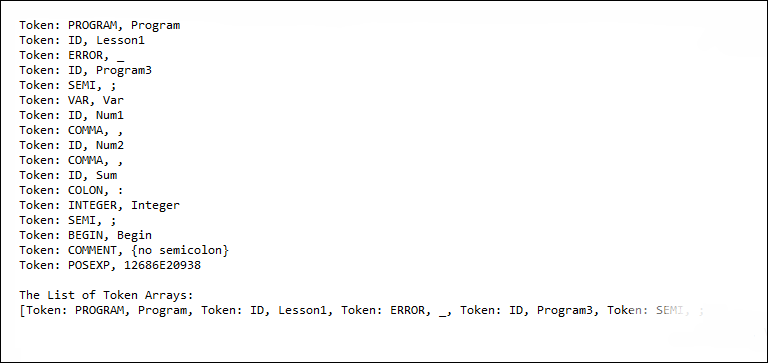
\includegraphics[width=1.1\textwidth]{output.PNG}
\end{center}
\caption{\label{Output}Token output to console}
\end{figure}


\subsection{Parser}

Not written

\subsection{Semantic Analysis}

Not written

\subsection{Code Generation}

Not written



\section{Change Log}

\begin{itemize}
\item
18 January 2017 - Miller - Created

\end{itemize}



\end{document}

